\documentclass[12pt]{article}
\usepackage[dvips]{graphics, color}
\begin{document}

\title{jsXe Design Notes}
\author{Ian Lewis}
\maketitle

\section{jsXe's UI}

\subsection{The TabbedView class}
jsXe's UI is designed with the \emph{TabbedView} class performing as the main
frame and container for jsXe's UI components. The TabbedView implements methods
to aid in the adding and removing of documents to jsXe's UI. The TabbedView
implements open documents an entries in a JTabbedPane that will allow the user
to switch between documents by clicking on the desired tab.

This class makes use of many action classes defined in the\\
$net.sourceforge.jsxe.actions$ package. One design goal is to eventually be able
to create actions "on the fly" using BeanShell scripting much the same way 
jEdit does. This allows new actions to be defined using a simple XML document
and once created the actions are loaded into an \emph{ActionSet} where they
can be easily referenced by name. This allows flexable support for easy
customization of toolbars and menus.

\subsection{The DocumentView interface}
Each tab contains an concrete instance of the \emph{DocumentView} interface.
DocumentViews are components that allow users to view an XML document in a
variety of ways. Each concrete Document view implements the DocumentView
interface. Thus the TabbedView and the rest of jsXe's classes do not deal with
the concrete interfaces. By creating this structure new XML document views can
be created easily.

\begin{figure}[h]
  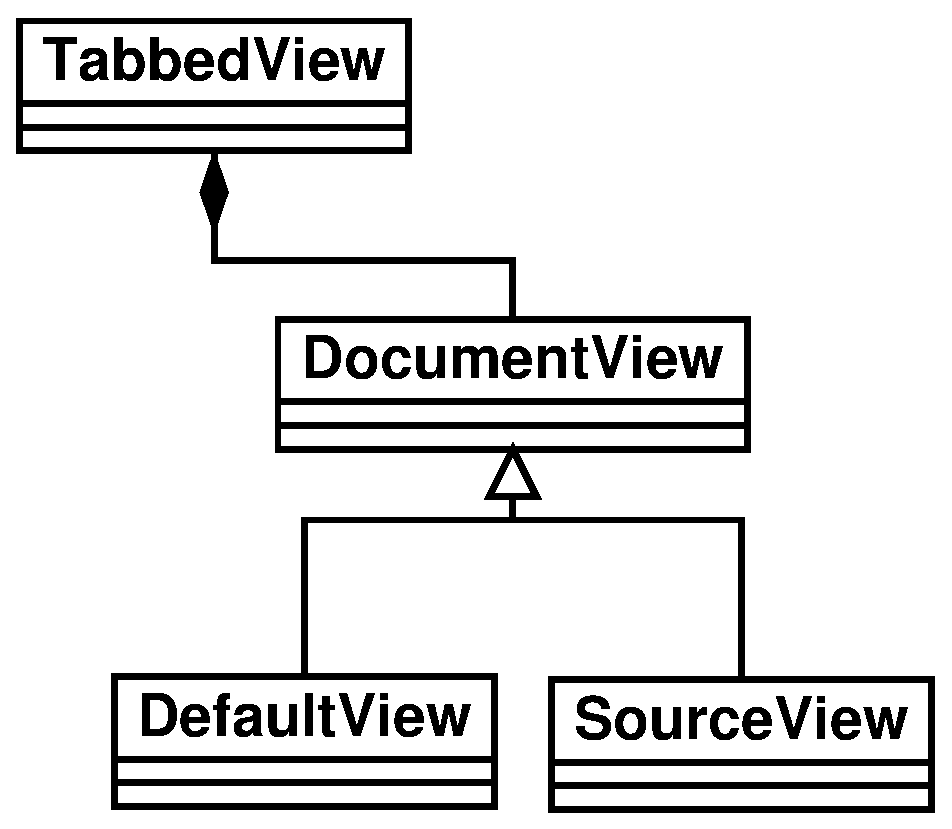
\includegraphics{uistructure.eps}
  \caption{\label{structure1}\emph{jsXe's UI class structure.}}
\end{figure}

Concrete DocumentView objects are created when documents are opened by
the \emph{DocumentViewFactory} class. This is done with the idea that some
criteria such as the type of the XML document might determine the view that is
returned. Also the interfaces of the concrete DocumentView
implementations can be encapsulated in this class.

\subsection{The DefaultView class}
This class is the default implementation of the \emph{DocumentView} interface. This
shows an XML document in a tree view.

\subsection{The SourceView class}
A pretty simple class that allows the user to edit the XML document as a text
file.

\section{jsXe's XML and DOM classes}

It's useful to look the Xerces-J API javadocs
( $http://xml.apache.org/xerces2-j/javadocs/api/index.html$ ) for reference when
reading the descriptions (and code) of the following classes.\\
\emph{Note: The design structures here are probobly the least well defined. They
could and probobly should be better.}

\subsection{The XMLDocument class}
The \emph{XMLDocument} class contains methods for interaction and editing of any
type of XML document. It provides methods for adding listeners to be notified
when the document changes and methods for editing the text of the XML document.
It was meant to be less application specific than the \emph{DocumentBuffer}
class which contains methods for finding out the file name on disk and logic for
dirty buffers (files edited the last save).

\subsection{The DefaultXMLDocument class}
The \emph{DefaultXMLDocument} class implements most of the methods in the
XMLDocument class. Since the DefaultXMLDocument implements methods that apply to
all types of XML documents the method implementations will probobly be pushed
into the XMLDocument class and DefaultXMLDocument will be made obsolete. Any
classes representing specific XML applications can then extend the XMLDocumnent
class.

The current DefaultXMLDocument really operates in two modes, parsed and
non-parsed. In parsed mode the document is assumed to be well-formed and the
model that is used is the Document object. In non-parsed mode the document is
not assumed to be well-formed and the text content is the model that is used.
This distinction is not visible to classes outside of the DefaultXMLDocument
class. One thing of note is that if changes are made to the underlying DOM then
the text will likely change thus making existing indeces into the document
invalid. Also if text is changed then any existing references that a user class
has will become invalid.\\
\emph{Note: This may not be the best design decision. An alternate design that
represents an XML document that can go from well-formed to non-wellformed and
back again is welcome. Perhaps one such as is used in Pollo where the document
being in parsed or non-parsed mode is visible to the rest of the application.}

\subsection{The AdapterNode class}
The AdapterNode is an adapter class that implements some methods that make
adding, removing, renaming and changing the value of org.w3c.dom.Node objects
easy. The Node interface sometimes requires a new Node object to be created
(when renaming the node for instance). This presents a problem since the Node
object is not persistent. The AdapterNode fortunately can be persistent and only
change the Node object it represents internally. It also implements an event
model that notifies listeners when the DOM is changed.

\subsection{The DOMSerializer class}
The \emph{DOMSerializer} class is what the DefaultXMLDocument class uses to
write the document to disk. This class is what really uses the DOM level 3
interfaces. There were no DOM2 interfaces that were adequate for serialization
and the old DOM1 XMLSerializer class was not an acceptable solution (it doesn't
respect whitespace within nodes and always formats (pretty-prints) the document
(see pollo bug report at\\{
\small
$http://sourceforge.net/tracker/index.php?func=detail\&aid=628167\&group\_id=30952\&atid=400872$}\\
for an explanation and example of a real user complaint).

\end{document}
